\documentclass[11pt]{article}

% ---------- Packages ----------
\usepackage[margin=1in]{geometry}
\usepackage{amsmath, amssymb}   % math
\usepackage{graphicx}           % \includegraphics
\usepackage{booktabs}           % nicer tables
\usepackage{float}              % [H] placement
\usepackage[font=small, skip=6pt]{caption}
\usepackage{xcolor}
\usepackage{listings}        % code blocks, pure TeX (no shell-escape)
\usepackage[hidelinks]{hyperref}

% ---------- Code block style (applies to every code block) ----------
% AVR assembly: listings ships no dialect for it, so define one.
\lstdefinelanguage{avrasm}{
  morekeywords={
    add,adc,sub,subi,sbc,sbci,and,andi,or,ori,eor,com,neg,inc,dec,tst,clr,ser,
    mov,movw,ldi,ld,ldd,lds,st,std,sts,push,pop,in,out,lpm,
    cp,cpc,cpi,cpse,breq,brne,brcs,brcc,brsh,brlo,brmi,brpl,brge,brlt,
    rjmp,jmp,ijmp,rcall,call,icall,ret,reti,nop,sleep,wdr,
    lsl,lsr,rol,ror,asr,swap,sbi,cbi,sbic,sbis,sbr,cbr,
  },
  morekeywords=[2]{.cseg,.dseg,.eseg,.org,.byte,.db,.dw,.equ,.def,.include,.macro,.endmacro},
  alsoletter={.},          % so directives like .cseg tokenize as one word
  morecomment=[l]{;},
  morestring=[b]",
  sensitive=false,
}
\lstdefinestyle{labcode}{
  basicstyle=\ttfamily\small,
  numbers=left, numberstyle=\tiny\color{gray!70}, numbersep=9pt,
  xleftmargin=2.2em, framexleftmargin=2.2em,   % background covers the number gutter
  breaklines=true, breakatwhitespace=true,
  frame=lines, framesep=2mm,
  backgroundcolor=\color{gray!8},
  keywordstyle=\color{blue!65!black}\bfseries,
  keywordstyle=[2]\color{purple!70!black},
  commentstyle=\color{green!40!black},
  stringstyle=\color{orange!85!black},
  showstringspaces=false,
  tabsize=4,
  captionpos=t,
}
\lstset{style=labcode}
\renewcommand{\lstlistingname}{Code}   % caption says "Code 1" instead of "Listing 1"

% ---------- Report info (edit these) ----------
\newcommand{\course}{ECE 3218L}
\newcommand{\labtitle}{Lab 3}
\newcommand{\studentname}{Daniel Xu}
\newcommand{\partners}{Manu Thomas}
\newcommand{\instructor}{Dr. Sternberg}
\newcommand{\labdate}{09/24/2026}

% article.cls always typesets title -> author -> date, so the date goes in the
% title block to sit directly under it. \date{} is required; empty means \today.
\title{\labtitle \\[0.3em] \large \labdate}
\author{\studentname \\ \small Partner: \partners \\ \small \course{} \,--\, \instructor}
\date{}

\begin{document}
\maketitle

\section{Overview}
Embedded systems and microcontrollers often interface with the real world through their input and output pins. This lab uses switches as inputs and LEDs as outputs on the Arduino board.


\section{Procedure}
\begin{enumerate}
\item A program that copies switch state to the LEDs.

The program configures PD2--PD7 as outputs for the LEDs and PC0--PC5 as inputs with pull-ups enabled, so an open switch reads as 1 and a closed switch as 0. The main loop reads \texttt{PINC}, keeps the lower six bits, shifts them left by two so that PC0 lines up with PD2, and writes the result to \texttt{PORTD}. Since the loop has no delay, the LEDs follow the switches immediately.

\item A program that rotates an LED from left to right.

After initializing the stack pointer, the program lights a single LED at PD2. Each step outputs the pattern, waits \texttt{STEP\_MS} milliseconds (using the delay loop subroutine), and shifts it left with \texttt{lsl}, moving the LED one position to the right. After the rightmost LED (PD7) stays lit for one step, the next shift leaves the register at zero; \texttt{flash\_all} then blinks all LEDs \texttt{FLASHES} times and the rotation restarts at PD2. The \texttt{delay\_ms} subroutine uses a 3999-iteration inner loop of 4 cycles per iteration, which together with the loop overhead gives 16\,000 cycles (1~ms at 16~MHz) per outer iteration.

\item A program that extends the previous one so that one of the switches selects the direction of rotation.

The program checks the switch on PC0 with \texttt{sbic} after every delay. When it is on (PC0~=~0), the LED moves left to right using \texttt{lsl}; when it is off, the LED moves right to left using \texttt{lsr}. Since the program checks the switch every step, flipping it reverses the LED mid-pass. A pass ends when the bit leaves the register (moving right) or drops below PD2 (moving left). All LEDs then flash, and \texttt{start\_pos} rereads the switch to start the next pass at PD2 or PD7.

\item A program that rotates a pattern obtained from switches, right to left.

The subroutine \texttt{read\_switches} reads PC0--PC5, inverts them with \texttt{com} so that an on switch lights its LED, and aligns them to PD2--PD7. Every \texttt{STEP\_MS} milliseconds the program displays the pattern and reads the switches again. If they changed, the new setting replaces the pattern; otherwise the program rotates the pattern one position. The rotation is circular: \texttt{lsr} shifts every bit towards PD2, \texttt{ori} wraps a bit leaving PD2 around to PD7, and \texttt{andi} clears the unused bits 0 and 1.
\end{enumerate}
Appendix~\ref{app:code} contains the full annotated listings: Program~1 in Code~\ref{code:copy}, Programs~2 and~3 in Code~\ref{code:rotate}, and Program~4 in Code~\ref{code:pattern}.

\section{Discussion}
\subsection{Circuit}
Figure~\ref{fig:circuit} shows the circuit on the course lab board. Jumper wires connect the Arduino header pins PC0--PC5 to the six toggle switches and PD2--PD7 to the LED bar, which has an on-board resistor network.

\begin{figure}[H]
  \centering
  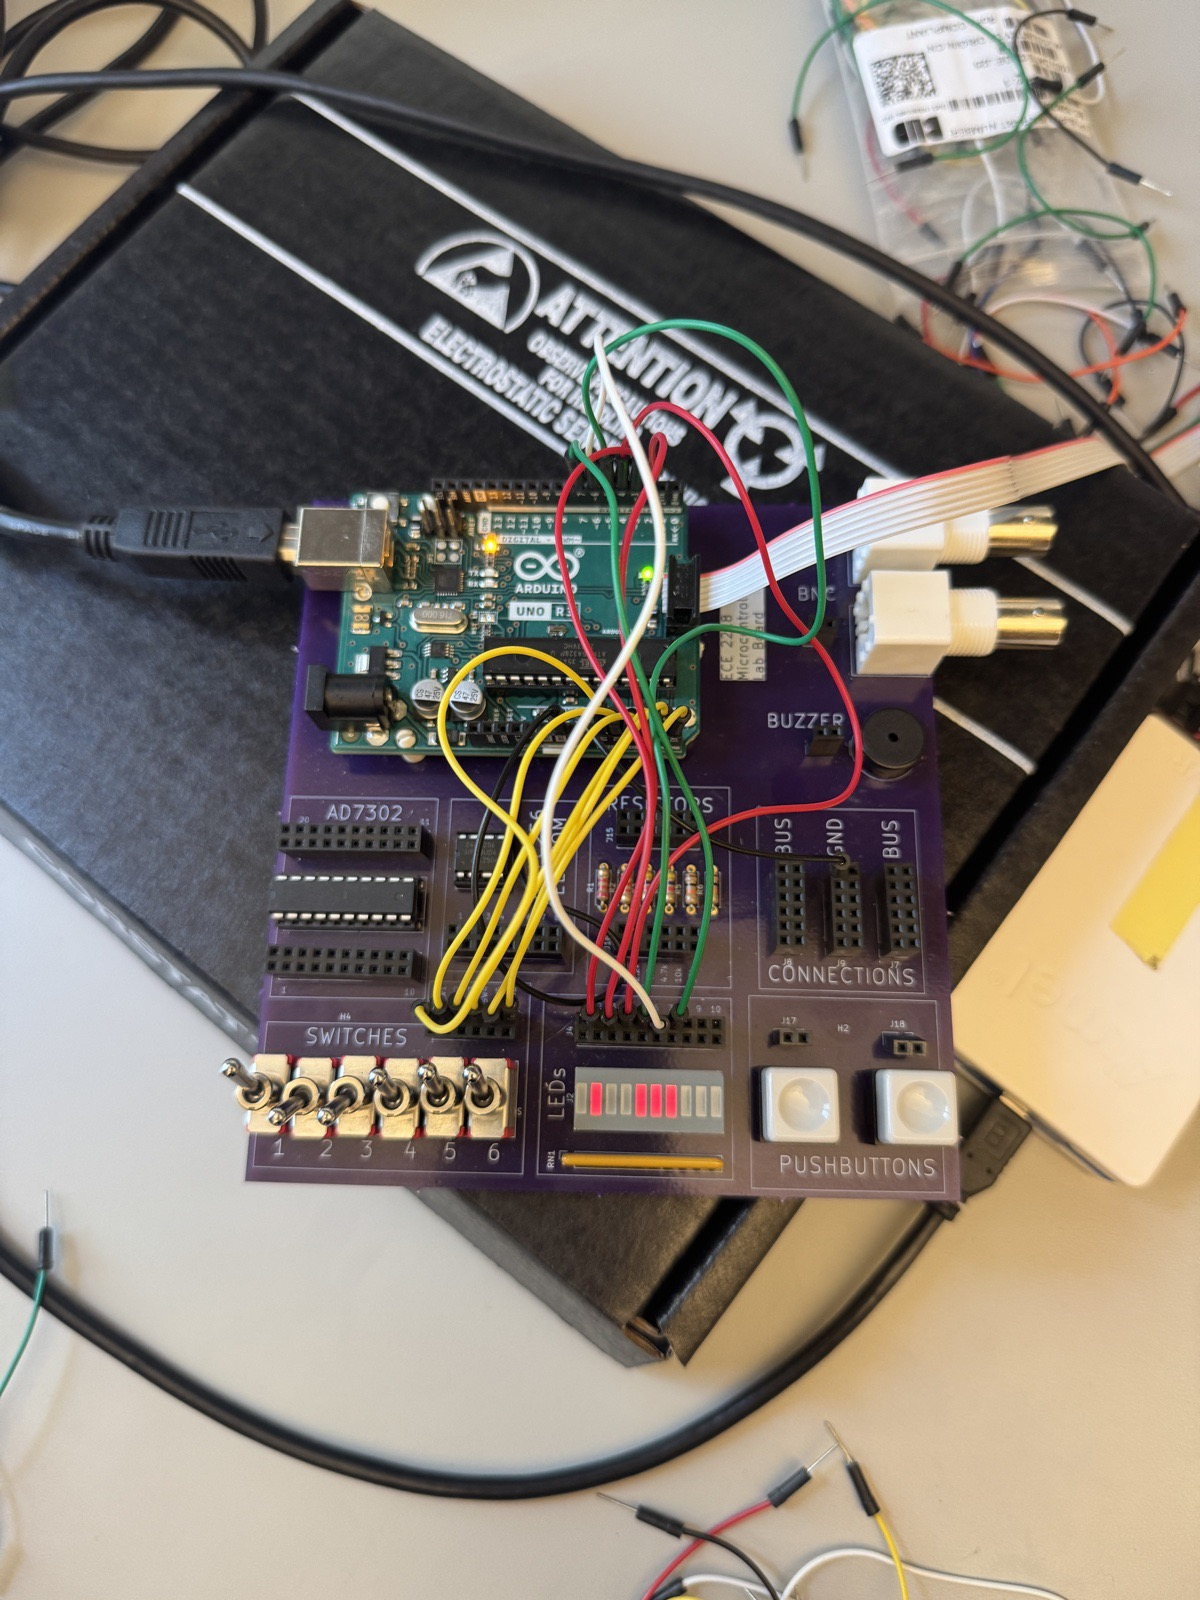
\includegraphics[width=0.6\textwidth]{circuit.jpg}
  \caption{Physical circuit on the lab board. The six toggle switches (bottom left) connect to PC0--PC5 and the LED bar (bottom center) to PD2--PD7.}
  \label{fig:circuit}
\end{figure}

PD2--PD7 drive the six LEDs directly, each in series with a 560~$\Omega$ resistor to ground, so an LED lights when its pin outputs a high level. The resistor limits the LED current. Assuming a forward voltage of about 2~V, each LED draws $(5 - 2)\,\text{V} / 560\,\Omega \approx 5.4$~mA, well below the 20~mA recommended and 40~mA absolute maximum current of an ATmega328P I/O pin. Without the resistor, only the output driver of the pin would limit the current, which could damage both the LED and the microcontroller.

The toggle switches connect PC0--PC5 to ground when closed. With the pins configured as inputs and their internal pull-up resistors enabled, an open switch reads as logic~1 and a closed switch as logic~0, so the switches are active low. Without the pull-ups, an open switch would leave the pin floating and \texttt{PINC} would return an undefined value.

\subsection{Mapping Inputs to Outputs}
Because the programs read the switches on PC0--PC5 but drive the LEDs on PD2--PD7, every program that copies switch data to the LEDs shifts it left by two bits.

Programs~2--4 place a \texttt{nop} between enabling the pull-ups and the first read of \texttt{PINC}. The input pins pass through a synchronizer, so a value written to \texttt{PORTC} does not appear in \texttt{PINC} until the following clock cycle.

\subsection{Delay Subroutine}
All timed programs use the same \texttt{delay\_ms} subroutine, which waits for the number of milliseconds passed in \texttt{r18}. Each outer iteration loads 3999 into \texttt{r25:r24} and decrements it with \texttt{sbiw}. With \texttt{sbiw} taking two cycles and a taken \texttt{brne} two cycles, one outer iteration takes
\begin{equation}
  2 + (4 \cdot 3999 - 1) + 1 + 2 = 16\,000 \text{ cycles},
\end{equation}
which is exactly 1~ms at 16~MHz. Including the \texttt{ldi} that loads the argument, \texttt{rcall} (3 cycles), \texttt{ret} (4 cycles), and the final \texttt{brne} that falls through, a call for $n$ milliseconds takes
\begin{equation}
  T_{\text{delay}}(n) = 16\,000\,n + 7 \text{ cycles}.
  \label{eq:delay}
\end{equation}

\section{After the Lab}
Lowering \texttt{STEP\_MS} in Program~2 until the eye could no longer follow the individual LEDs lighting up one after another gave a final value of \texttt{STEP\_MS}~=~2.

One step of the left-to-right rotation executes \texttt{out} (1 cycle), the delay call of Eq.~\eqref{eq:delay}, \texttt{sbic} skipping the next instruction (2 cycles), \texttt{lsl} (1 cycle), and a taken \texttt{brne} (2 cycles):
\begin{equation}
  T_{\text{step}} = 1 + (16\,000 \cdot 2 + 7) + 2 + 1 + 2 = 32\,013 \text{ cycles} = \frac{32\,013}{16 \times 10^{6}\ \text{Hz}} \approx 2.0008 \text{ ms}.
\end{equation}
Each LED therefore stays lit for about 2~ms. A full pass across the six LEDs takes about 12~ms, and the boundary flash (all LEDs on for \texttt{STEP\_MS}, then off for \texttt{STEP\_MS}) adds another 4~ms, so the whole pattern repeats every 16~ms (62.5~Hz).

Table~\ref{tab:timing} compares this timing with the nominal 200~ms delay.

\begin{table}[H]
  \centering
  \caption{Program 2 timing at 16 MHz with \texttt{FLASHES} = 1.}
  \label{tab:timing}
  \begin{tabular}{lrr}
    \toprule
    Quantity & \texttt{STEP\_MS} = 200 & \texttt{STEP\_MS} = 2 \\
    \midrule
    Time each LED is lit       & 200.0 ms & 2.0 ms \\
    One pass over 6 LEDs       & 1.2 s    & 12 ms \\
    Pass plus boundary flash   & 1.6 s    & 16 ms \\
    Repetition rate            & 0.63 Hz  & 62.5 Hz \\
    \bottomrule
  \end{tabular}
\end{table}

At 2~ms per step, all of the LEDs appear lit at the same time: each LED turns on and off 62.5 times per second, fast enough that the human eye perceives a steady light.

\section{Conclusion}
In this lab, the ATmega328P drove six LEDs on PORTD and read six toggle switches on PORTC. The data direction registers configure the pins, and the internal pull-up resistors make the active-low switches readable without external components. The programs copy the switches to the LEDs, rotate a single LED with a direction selected by a switch and a flash at the boundary, and rotate a pattern entered on the switches. A cycle-counted delay subroutine provides an exact 1~ms time base. Reducing the step delay to 2~ms made the individual LEDs indistinguishable, with the full pattern repeating at 62.5~Hz.

\appendix
\section{Full Code}
\label{app:code}

% ----- Code block: paste code between \begin{lstlisting} and \end{lstlisting} -----
\begin{lstlisting}[language=avrasm,caption={Program 1. Copies switch state to the LEDs.},label={code:copy}]
.def temp = r16

.cseg
.org 0x0000
        rjmp reset

reset:
        ldi  temp, 0b11111100
        out  DDRD, temp             ; PD7..PD2 outputs
        clr  temp
        out  PORTD, temp            ; all LEDs off
        out  DDRC, temp             ; PC0..PC5 inputs
        ldi  temp, 0b00111111
        out  PORTC, temp            ; enable pull-ups on PC0..PC5

main:
        in   temp, PINC             ; read switches
        andi temp, 0b00111111       ; keep only PC0..PC5
        lsl  temp                   ; PC0 -> PD1 position
        lsl  temp                   ; PC0 -> PD2 position
        out  PORTD, temp            ; show on LEDs
        rjmp main                   ; repeat forever
\end{lstlisting}

\begin{lstlisting}[
    language=avrasm,
    caption={Program 2/3. Rotating LEDs in a direction selected by a switch.},
    label={code:rotate}
    ]
.equ STEP_MS   = 200                ; time each LED is lit (1..255 ms)
.equ FLASHES   = 1                  ; number of flashes at the boundary
.equ DIR_BIT   = 0                  ; direction switch on PC0
.equ LEDS_ALL  = 0b11111100         ; PD7..PD2
.equ LED_LEFT  = 0b00000100         ; PD2 = leftmost LED
.equ LED_RIGHT = 0b10000000         ; PD7 = rightmost LED

.def temp  = r16
.def cnt   = r18                    ; delay_ms argument
.def led   = r20                    ; current LED pattern
.def nflsh = r21

.org 0x0000
        rjmp reset

reset:
        ldi  temp, high(RAMEND)     ; stack pointer (needed for rcall)
        out  SPH, temp
        ldi  temp, low(RAMEND)
        out  SPL, temp

        ldi  temp, LEDS_ALL
        out  DDRD, temp             ; PD7..PD2 outputs
        clr  temp
        out  DDRC, temp             ; PORTC inputs
        ldi  temp, 0b00111111
        out  PORTC, temp            ; pull-ups on PC0..PC5
        nop                         ; input synchronizer delay before 1st read

        rcall start_pos             ; pick starting end from the switch

step:
        out  PORTD, led             ; light the current LED
        ldi  cnt, STEP_MS
        rcall delay_ms              ; wait STEP_MS ms
        sbic PINC, DIR_BIT          ; PC0 = 0 (switch ON)? skip next
        rjmp go_left                ; PC0 = 1 (switch OFF) -> right to left

go_right:                           ; left to right: PD2 -> PD7
        lsl  led
        brne step                   ; after PD7 the bit falls out -> 0
        rjmp boundary

go_left:                            ; right to left: PD7 -> PD2
        lsr  led
        cpi  led, LED_LEFT
        brsh step                   ; still at PD2 or higher -> continue

boundary:                           ; light left the 6 LEDs
        rcall flash_all
        rcall start_pos
        rjmp step

; start_pos: led = PD2 if moving right, PD7 if moving left
start_pos:
        ldi  led, LED_LEFT          ; assume left to right: start at PD2
        sbic PINC, DIR_BIT          ; switch ON -> keep PD2
        ldi  led, LED_RIGHT         ; switch OFF -> start at PD7
        ret

flash_all:
        ldi  nflsh, FLASHES
fa_loop:
        ldi  temp, LEDS_ALL
        out  PORTD, temp            ; all on
        ldi  cnt, STEP_MS
        rcall delay_ms
        clr  temp
        out  PORTD, temp            ; all off
        ldi  cnt, STEP_MS
        rcall delay_ms
        dec  nflsh
        brne fa_loop
        ret

; delay_ms: wait r18 milliseconds (1..255) at 16 MHz
;   one ms = 2 + (4*3999 - 1) + 1 + 2 = 16000 cycles
;   total  = 16000*n + 7 cycles incl. ldi, rcall, ret
delay_ms:
dm_outer:
        ldi  r24, low(3999)
        ldi  r25, high(3999)
dm_inner:
        sbiw r24, 1
        brne dm_inner
        dec  cnt
        brne dm_outer
        ret
\end{lstlisting}

\begin{lstlisting}[
    language=avrasm,
    caption={Program 4. Rotating a pattern obtained from switches.},
    label={code:pattern}
    ]
.equ STEP_MS   = 200                ; time per step (1..255 ms)
.equ LEDS_ALL  = 0b11111100         ; PD7..PD2
.equ LED_RIGHT = 0b10000000         ; PD7 = rightmost LED

.def temp    = r16
.def cnt     = r18                  ; delay_ms argument
.def pattern = r20                  ; pattern as shown on PORTD
.def last    = r21                  ; last switch value read

.org 0x0000
        rjmp reset

reset:
        ldi  temp, high(RAMEND)     ; stack pointer (needed for rcall)
        out  SPH, temp
        ldi  temp, low(RAMEND)
        out  SPL, temp

        ldi  temp, LEDS_ALL
        out  DDRD, temp             ; PD7..PD2 outputs
        clr  temp
        out  DDRC, temp             ; PORTC inputs
        ldi  temp, 0b00111111
        out  PORTC, temp            ; pull-ups on PC0..PC5
        nop                         ; input synchronizer delay before 1st read

        rcall read_switches         ; initial pattern
        mov  pattern, temp
        mov  last, temp

loop:
        out  PORTD, pattern         ; show the pattern
        ldi  cnt, STEP_MS
        rcall delay_ms              ; wait STEP_MS ms

        rcall read_switches         ; did the switches change?
        cp   temp, last
        breq rotate
        mov  last, temp             ; yes -> load the new pattern
        mov  pattern, temp
        rjmp loop

rotate:                             ; 6-bit circular rotate PD7 -> PD2
        lsr  pattern                ; every bit moves one LED to the left;
                                    ; the bit that was on PD2 lands in bit 1
        sbrc pattern, 1             ; did a bit fall off the left end (PD2)?
        ori  pattern, LED_RIGHT     ; yes -> wrap it around to PD7
        andi pattern, LEDS_ALL      ; clear bit 1 (and bit 0)
        rjmp loop

read_switches:
        in   temp, PINC
        com  temp                   ; closed switch = 0 -> make it 1
        andi temp, 0b00111111       ; keep only PC0..PC5
        lsl  temp
        lsl  temp                   ; PC0..PC5 -> PD2..PD7
        ret

delay_ms:
dm_outer:
        ldi  r24, low(3999)
        ldi  r25, high(3999)
dm_inner:
        sbiw r24, 1
        brne dm_inner
        dec  cnt
        brne dm_outer
        ret
\end{lstlisting}

\end{document}